%----------------------------------------------------------------------------------------
%	PACKAGES AND OTHER DOCUMENT CONFIGURATIONS
%----------------------------------------------------------------------------------------

\documentclass[paper=a4, fontsize=11pt]{scrartcl} % A4 paper and 11pt font size

% ---- Entrada y salida de texto -----

\usepackage[T1]{fontenc} % Use 8-bit encoding that has 256 glyphs
\usepackage[utf8]{inputenc}
%\usepackage{fourier} % Use the Adobe Utopia font for the document - comment this line to return to the LaTeX default

% ---- Idioma --------

\usepackage[spanish, es-tabla]{babel} % Selecciona el español para palabras introducidas automáticamente, p.ej. "septiembre" en la fecha y especifica que se use la palabra Tabla en vez de Cuadro

% ---- Otros paquetes ----
\usepackage{csquotes} %Para permitir el uso de comillas Quotes https://tex.stackexchange.com/questions/36812/isnt-there-any-other-way-of-doing-double-quotes-in-latex-besides
\usepackage[hyphens]{url} % ,href} %para incluir URLs e hipervínculos dentro del texto (aunque hay que instalar href)
\usepackage{hyperref}
\usepackage{color}
\usepackage{graphics,graphicx, floatrow} %para incluir imágenes y notas en las imágenes
\usepackage{graphics,graphicx, float} %para incluir imágenes y colocarlas

\graphicspath {{./img/}}

\usepackage{listings}  %para introducir comandos

\lstdefinestyle{mybash}
{basicstyle=\ttfamily,
  showstringspaces=false,
  commentstyle=\color{red},
  keywordstyle=\color{blue},
  language=bash,
  alsoletter=/,
  basicstyle=\footnotesize,
  numbers=left,
  stepnumber=1,
  showstringspaces=false,
  tabsize=1,
  breaklines=true,
  breakatwhitespace=false,
}
\lstdefinestyle{mysql}
{basicstyle=\ttfamily,
  showstringspaces=false,
  commentstyle=\color{red},
  keywordstyle=\color{blue},
  language=sql,
  basicstyle=\footnotesize,
  numbers=left,
  stepnumber=1,
  showstringspaces=false,
  tabsize=1,
  breaklines=true,
  breakatwhitespace=false,
}


% Para hacer tablas comlejas
%\usepackage{multirow}
%\usepackage{threeparttable}

%\usepackage{sectsty} % Allows customizing section commands
%\allsectionsfont{\centering \normalfont\scshape} % Make all sections centered, the default font and small caps

\usepackage{fancyhdr} % Custom headers and footers
\pagestyle{fancyplain} % Makes all pages in the document conform to the custom headers and footers
\fancyhead{} % No page header - if you want one, create it in the same way as the footers below
\fancyfoot[L]{} % Empty left footer
\fancyfoot[C]{} % Empty center footer
\fancyfoot[R]{\thepage} % Page numbering for right footer
\renewcommand{\headrulewidth}{0pt} % Remove header underlines
\renewcommand{\footrulewidth}{0pt} % Remove footer underlines
\setlength{\headheight}{13.6pt} % Customize the height of the header

\setlength\parindent{0pt} % Removes all indentation from paragraphs - comment this line for an assignment with lots of text

\newcommand{\horrule}[1]{\rule{\linewidth}{#1}} % Create horizontal rule command with 1 argument of height


%----------------------------------------------------------------------------------------
%	TÍTULO Y DATOS DEL ALUMNO
%----------------------------------------------------------------------------------------
\graphicspath{ {img/} }

\title{
\normalfont \normalsize
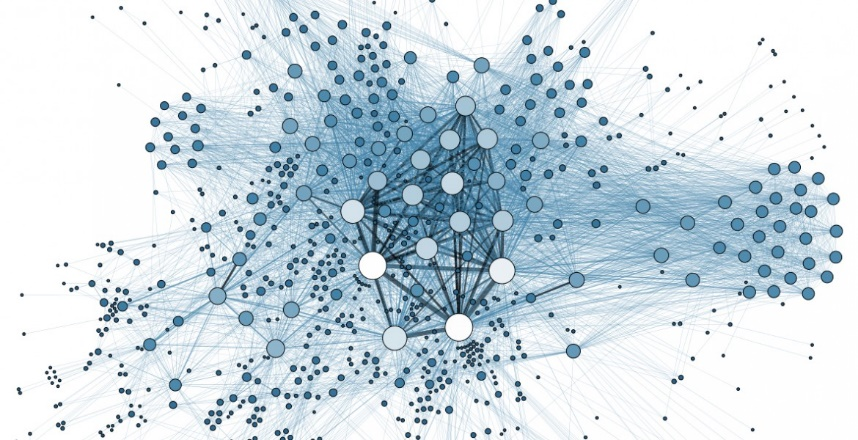
\includegraphics[width=13cm,height=6cm]{portada}\\
\textsc{\textbf{Algorítmica (2022-2023)} \\ Grado en Ingeniería Informática \\ Universidad de Granada} \\ [25pt] % Your university, school and/or department name(s)
\horrule{0.5pt} \\[0.4cm] % Thin top horizontal rule
\huge Memoria Práctica 3 \\ % The assignment title
\horrule{2pt} \\[0.5cm] % Thick bottom horizontal rule
}

%https://es.overleaf.com/learn/latex/Inserting_Images
%Ruta relativa de   imagenes

\author{Pedro Antonio Mayorgas Parejo  \\  Alejandro Ramos Peña} % Nombre y apellidos

\date{\normalsize\today} % Incluye la fecha actual

%----------------------------------------------------------------------------------------
% DOCUMENTO
%----------------------------------------------------------------------------------------

\begin{document}

\maketitle % Muestra el Título

\newpage %inserta un salto de página

\tableofcontents % para generar el índice de contenidos

\newpage

%----------------------------------------------------------------------------------------
%	Cuestión 1
%----------------------------------------------------------------------------------------

\section{Componentes del algoritmo Greedy}
Como ya sabemos, un algoritmo greedy tiene que estar formado de distintos elementos para poder ser formalizado como tal.
\vspace{5mm}

En este algoritmo tenemos los siguientes elementos:
\begin{itemize}
    \item \textbf{Conjunto de candidatos:} En este caso, el conjunto de candidatos es el conjunto de aristas del grafo.
    \item \textbf{Conjunto de seleccionados:} El conjunto de seleccionados es el conjunto de nodos que forman el camino euleriano.
    \item \textbf{Función de selección:} La función de selección es la que nos va a permitir elegir la arista que vamos a añadir al camino. En este caso, la función de selección es la que nos va a permitir elegir el nodo al que vamos a saltar.
    \item \textbf{Función de factibilidad:} Es la función que comprueba si se puede obtener una solución. En este caso es la función que comprueba los prerrequisitos de un camino euleriano en un grafo.
    \item \textbf{Función solución:} La función solución es la que nos va a permitir comprobar si hemos llegado al final del camino. En este caso, la función objetivo es la que comprueba si queda alguna arista en el nodo actual.
    \item \textbf{Funcion objetivo:} Es la función que devuelve el camino euleriano. En este caso es la función que devuelve el contenido de la variable de camino.
\end{itemize}

\section{Descripción del algoritmo Greedy con heurística basada en la matriz de adyacencia}

El algoritmo está encapsulado en una clase, debido a las enormes necesidades de heurística del algoritmo greedy.
\vspace{5mm}

La heurística de este algoritmo es basada en la matriz de adyacencia, donde la matriz de adyacencia nos proporciona información sobre las aristas de los vértices (o nodos) del grafo, a partir de la entrada de la matríz de adyacencia construimos la siguiente información:

\begin{itemize}
    \item Obtenemos los grados de cada vértice del grafo. Por grado, es la cantidad de aristas que tiene, contabilizadas mediante, la matriz.
    \item Obtenemos los puntos iniciales, si en la matriz hay dos vértices con grado impar, se debe empezar en uno de los dos y acabar en el otro punto.
    \item Del fichero de entrada obtenemos el número de nodos.
\end{itemize}

Una vez obtenida toda la heurísitca ejecutamos el método \textbf{fleuryAlgorithm}, el algoritmo se ejecuta en base a lo siguiente:
\vspace{5mm}

\textbf{El algoritmo está preparado para obtener todas las posibles rutas desde todos los vértices.} 
\vspace{5mm}

Se hace una copia de la matriz de adyacencia original y de los grados de los vértices, para no perder la información de la adyacencia durante las distintas búsquedas de rutas.
\vspace{5mm}

Pero debido a los limitados requisitos de la práctica solo se hará desde un punto, que se limita en la función de evalIfEulerPath, en dicha función se ha preparado que cuando los nodos sean pares, se introduzca un par aleatorio a partir del atributo de instancia del número de nodos.

\begin{enumerate}
    \item Si la matriz tiene un solo nodo, se introduce el nodo y se termina la función.
    \item Si la matriz tiene mas de un nodo, el algoritmo obtiene el nodo de partida (este ha sido obtenido previamente en evalIfEulerPath y lo almacena en una variable temporal que indexa el vértice en el que está evaluando el siguiente al que debe saltar.
    \item Se introduce el nodo inicial en el eulerPath, para almacenar el nodo de partida.
    \item Evalúa si el nodo actual tiene un grado mayor que 0, si no lo tiene se termina el bucle y la función. 
    \item En caso de tener un grado mayor de 0, pasamos a recorrer su matriz de adyacencia, evaluando las siguientes condiciones básicas en todos los requisitos.
    \begin{itemize}
        \item El siguiente vértice, debe tener una arista, esto es que en la matriz de adyacencia vale 1. Una vez evaluado esto, debemos evaluar las siguientes subcondiciones.
        \begin{itemize}
            \item Si el siguiente vértice tiene una arista y un grado igual a 1, se almacena como el posible Dead end. A continuacuón evaluamos los siguientes puntos.
            \item Si el siguiente vértice tiene una arista y un grado mayor que 1, evaluamos a continuación si este tiene un grado 2, para evaluar que no conduzca a otro posible Dead end, esto es que cuando saltemos al siguiente vértice y construyamos el siguiente camino. Que su siguiente salto a su vez no tenga grado 1, esto es evitando vértices que en el grafo no tienen salida y dejen sin evaluar el resto de vértices. Si este punto conduce a un DeadEnd se almacena también como posible salto y pasamos a evaluar al resto de vértices. 
            
            En caso contrario, si el siguiente vértice tiene un grado mayor que 1, lo escogemos directamente como salto válido.
            \item Si el siguiente vértice tiene un grado mayor que 2, es un vértice bueno y lo seleccionamos directamente como siguiente salto.
        \end{itemize}

        \item Si se ha cumplido con una subcondición de dead end y hemos evaluado todos los posibles vértices. Comprobamos cuál tipo de dead end es, si es un dead end de dos saltos esto es que el siguiente vértice tiene otro siguiente vértice que conduce a un final del grafo, escogemos ese en primer lugar para construir el camino. Si no hay uno de dos saltos, se escoge como siguiente el vértice que conduce a un final.
    \end{itemize}
\end{enumerate}

Una vez completada la evaluación, con ese vértice de salto, pasamos a modificar la matriz para notificar que el salto se ha realizado, además se decrementa el grado de dicho vértice, para que en las próximas evaluaciones se escoja el mejor camino posible.
\vspace{5mm}

Finalmente se marca como vértice actual el del salto, se reinician las variables de lo vértices de salto, los de dead end y se añade al camino el vértice del salto. Repetimos la iteración evaluando de nuevo las condiciones anteriores a partir de la matriz de adyacencia del nuevo vértice actual para producir el siguiente salto.
\vspace{5mm}

Una vez que todos los puntos hayan recorrido al menos 1 vez todo el grafo, el bucle termina cuando el grado del último vértice vale 0, esto es ha sido el último.
\vspace{5mm}

Luego dependiendo de si queremos evaluar otros caminos, se reinicia la matriz de adyacencia y la de grados. Para empezar de nuevo si hay otro camino que evaluar desde otro vértice.

\newpage
\section{Algoritmo con heurística de número de aristas incidentes.}

La heurística de este algoritmo se basa en coger el primer nodo adyacente al actual en el cual inciden más aristas. De este modo, conseguimos que el algoritmo se dirija hacia los nodos que tienen más aristas incidentes, y por tanto, más posibilidades de que el algoritmo no se quede sin opciones de camino.
\vspace{5mm}

Para pasarle como argumento al programa un grafo hemos especificado un formato de archivo .graph de texto que especifica un grafo donde:

\begin{enumerate}
    \item La primera línea tiene que contener la letra G para que se compruebe que el formato del archivo es correcto
    \item La segunda línea indica el número de nodos del grafo.
    \item Las siguientes líneas indican las aristas del grafo, donde cada línea tiene primero el número de aristas que tiene el nodo y despúes todos los nodos a los que está conectado, de 0 a n-1.
\end{enumerate}

Además, hemos creado una clase Nodo con distintos métodos que nos van a permitir ir eliminando aristas conforme vayamos recorriendo el grafo y poder obtener el número de aristas incidentes fácilmente
\vspace{5mm}

Una vez hemos leído el grafo y lo hemos almacenado en un vector de Nodos, se ejecuta el algoritmo de la siguiente manera:
\begin {enumerate}
    \item Mientras que el nodo actual tenga alguna arista incidente:
    \begin{enumerate}
        \item Comprobamos de todos los Nodos adyacentes cual es el que tiene un mayor número de aristas incidentes para saber cuál es el siguiente.
        \item Añadimos el nodo actual al camino
        \item Se elimina la arista que une el nodo actual con el nodo siguiente.
        \item Se actualiza el nodo actual al nodo adyacente.
    \end {enumerate}
    \item Una vez que el nodo actual no tiene aristas incidentes, se añade al camino y se termina el algoritmo.
\end {enumerate}

\newpage
\section{Eficiencia de los algoritmos}

\subsection{Algoritmo basado en heurística de matriz de adyacencia}
La complejidad viene dada por la visita de todos los posibles vértices del grafo, así como la evaluación del vector de grados, para evaluar cuál es el siguiente punto.

Siendo N el número de Vértices que tiene que analizar y E² los dos vectores de heurística del grado de los vértices de origen y el de destino.

\textbf{Complejidad en el peor caso: O(N+E²).}

\subsection{Algoritmo basado en heurística de aristas incidentes.}
Este algoritmo es más sencillo y fácil de implementar que el que usa como heurística la matriz de adyacencia, pero es menos eficiente, ya que en el peor caso, que es cuando todos los nodos están conectados con todos entre sí, \textbf{la complejidad es O(n²)}, ya que en cada iteración del bucle principal (aunque se vayan eliminando aristas) se recorren todos los nodos adyacentes para encontrar el nodo con más aristas incidentes.


\newpage

\section {Cómo compilar y ejecutar la aplicación}

Para compilar la aplicación, se debe ejecutar el comando siguiente en la carpeta raíz del proyecto. Esto generará dos ejecutables, arista.bin y adjacency.bin.

\begin{lstlisting}[style=mybash]
# On project root
make run
# Or build and manual running
make build
# run matrix adjacency heuristic
./adjacency.bin salida.txt adjacencymatrix.matrix
# run edge heuristic
./arista.bin grafoEjemplo.graph
\end{lstlisting}

Como parámetros de entrada tienen:
\begin{itemize}
    \item \textbf{arista.bin}: El nombre del archivo de texto que contiene el grafo.
    \item \textbf{adjacency.bin}: El nombre del archivo de texto para la salida y después el nombre del fichero de texto que contiene el grafo de adyacencia.
\end{itemize}

Además se pueden ejecutar ambos con el grafo de las diapositivas de la práctica con el comando \textbf{make run} y con otro grafo de ejemplo. 

\newpage
\section{Ejecución del ejercicio 1}

\begin{figure}[H]
	\centering
	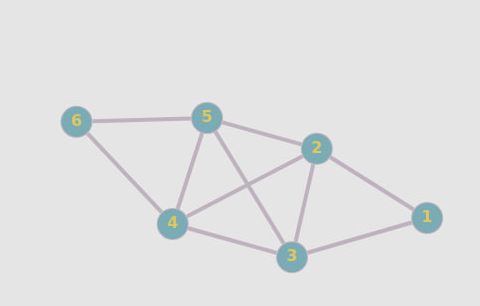
\includegraphics[scale=0.40]{grafo_ejercicio1}
	\caption{Grafo del ejercicio 1 el ejemplo propuesto}
\end{figure}

\textbf{Heurística de matriz de adyacencia}

\begin{figure}[H]
	\centering
	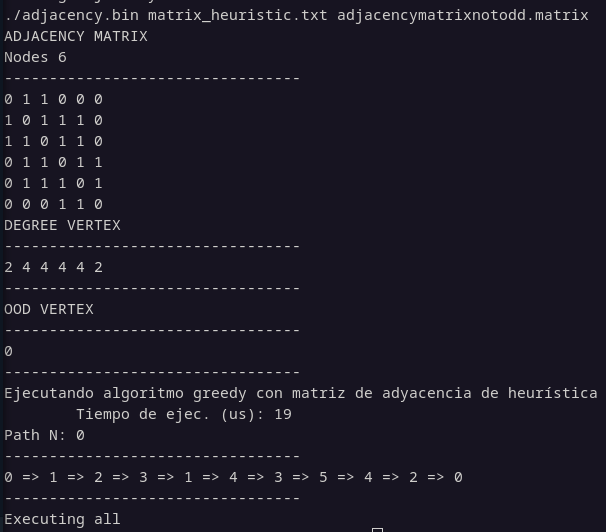
\includegraphics[scale=0.40]{adjacency1}
	\caption{Heurística de matriz de adyacencia aplicadas al grafo 1}
\end{figure}

\textbf{Heurística de aristas }

\begin{figure}[H]
	\centering
	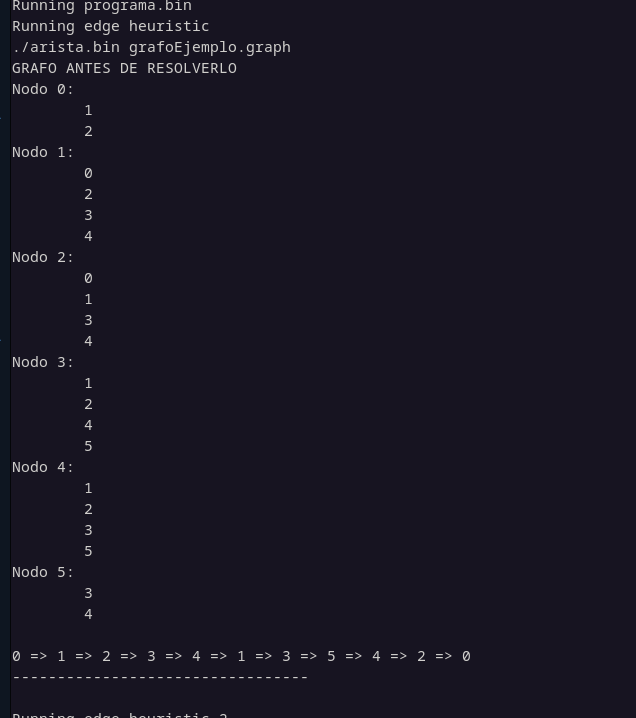
\includegraphics[scale=0.40]{edge1}
	\caption{Heurística de aristas aplicadas al grafo 1}
\end{figure}

\newpage
\section{Ejecución del ejercicio 2}

\begin{figure}[H]
	\centering
	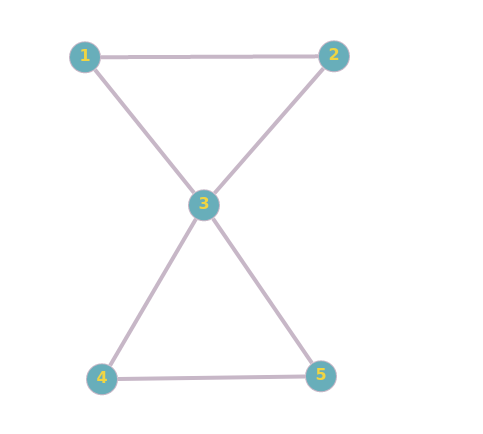
\includegraphics[scale=0.40]{grafo_ejercicio2}
	\caption{Grafo del ejercicio 2}
\end{figure}

\textbf{Heurística de matriz de adyacencia}

\begin{figure}[H]
	\centering
	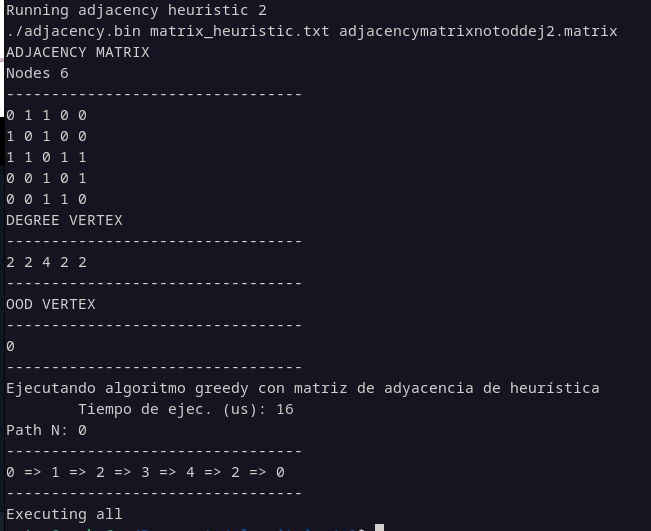
\includegraphics[scale=0.40]{adjacency2}
	\caption{Heurística de matriz de adyacencia aplicadas al grafo 2}
\end{figure}

\textbf{Heurística de aristas }

\begin{figure}[H]
	\centering
	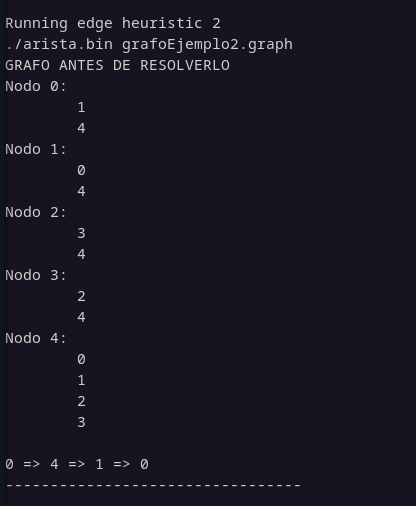
\includegraphics[scale=0.40]{edge2}
	\caption{Heurística de aristas aplicadas al grafo 2}
\end{figure}

% \begin{lstlisting}[style=mybash]
%     # Para una base de datos concreta
%     mysqldump --user=tiendabd --password=password --databases tiendabd --add-drop-database --add-drop-table [--replace] --host=127.0.0.1 --result-file=dump.sql
% \end{lstlisting}



%\begin{figure}[H]
%	\centering
%	\includegraphics[scale=0.30]{cuestion_1_1}
%	\caption{Se puede ver que al no haber un fallo grave, el sistema lo nota como que sigue funcionando pero en un estado degradado.}
%\end{figure}

%\newpage

%Se pueden hacer include en latex
%\newpage

\section{Section}

\subsection{Subseccion}

\subsubsection{Subseccion}



%-------Bibliografia-----------------------------

%\newpage
\section{Bibliografía}

% Ejemplo
\footnote{Administración de mdadm - Por Red Hat}
\textcolor{blue}{\url{https://access.redhat.com/documentation/en-us/red_hat_enterprise_linux/8/html/managing_storage_devices/managing-raid_managing-storage-devices#monitoring-raid_managing-raid}}



\end{document}
